\documentclass[portrait,a0,final]{a0poster} % a0poster class sets the paper size
\usepackage[RGB,A0]{ScientificPosterTemplate} % RGB, Coated, Uncoated
\usepackage[english]{babel}
\usepackage[pdftex]{graphicx}
\usepackage{epstopdf} % so that ''pdflatex'' accepts .eps files
\usepackage{titlesec} % For changing the font on chapters, sections, etc.
\usepackage{multirow}
\usepackage[table]{xcolor}
\usepackage{tabularx}
\usepackage{lipsum} % Lorem ipsum generator
\usepackage{floatrow}


\definecolor{bleu}{RGB}{0,140,189}%

%% Section font size reduction for a0 posters %%%%%%%%%%%%%%%%%%%%%%%%%%%%%%%%%%%%%%%%%

% \titleformat{\section}{\large\bfseries\sffamily\color{posterBlack}}{\textcolor{posterBlack}{\thesection}}{1em}{} % Text size for a1 posters
% \titleformat{\section}{\large\bfseries\sffamily}{\thesection.}{1em}{} % Text size for a1 posters with a dot after the incremental number
\titleformat{\section}{\huge\bfseries\sffamily\color{bleu}}{\textcolor{bleu}{\thesection.}}{1em}{} % Text size for a1 posters with a dot after the incremental number

%% Safe alternative math font (optional)
% \usepackage{fouriernc}

%% Teach hyphenation for alien words
% \hyphenation{op-tical net-works semi-conduc-tor}


%% Font sizes for a0poster are
%\tiny
%\scriptsize
%\footnotesize
%\small
%\normalsize
%\large
%\Large
%\LARGE
%\huge
%\Huge
%\veryHuge
%\VeryHuge
%\VERYHuge

%% Colors from ScientificPosterTemplate-package
% posterBlack
% posterGray
% posterYellow
% posterOrange
% posterRed
% posterFuchsia
% posterPurple
% posterBlue
% posterTurquoise
% posterGreen
% posterLightGreen
% You can use \textcolor{<posterColor>}{<your text>) to change the colors of text

%%%%%%%%%%%%%%%%%%%%%%%%%%%%%%%%%%%%%%%%%%%%%%%%%%%%%%%%%%%%%%%%%%%%%%%%%%%%%%%%%%%%%%%










\begin{document}



\thispagestyle{empty} % Removes the page number

\begin{minipage}[t]{0.98\linewidth} % The first minipage for the logo & title
\vspace{0pt} % A trick to align the parallel minipages on top

\vspace{0.008\linewidth} % Increase the top margin

\begin{minipage}[t]{0.95\linewidth} % title
\vspace{0pt} % Alingns the parallel minipages on top

%% Title: use \baselinestretch to change linespacing, \textit{} for italic text, \textcolor for colored text
% More conservative title, upright and black
{\renewcommand{\baselinestretch}{0.85} % Changes the baseline skip smaller for the title
\VeryHuge{\bfseries{\textsf{\textcolor{bleu}{Towards a better predictive model
from rest fMRI: benchmarks across multiple phenotypes}}}} % Text size for a1 posters
\par} % <- for \baselinestretch

\vspace{0.02\linewidth} % Empty space after the title

\Large{\textsf{\bfseries{\underline{Kamalaker Dadi}$^{1*}$, Darya Chyzhyk$^1$,
Alexandre Abraham$^1$, Mehdi Rahim$^1$, Bertrand Thirion$^1$,
Gael Varoquaux$^1$}}} % Text size for a1 posters

\vspace{0.01\linewidth}
\Large{\textcolor{posterBlack}{\textsf
}}}
%
\end{minipage}
\hspace{0.08\linewidth}
%\begin{minipage}{0.15\linewidth} % logo
%\vspace{0pt} % Alingns the parallel minipages on top
%\begin{flushright}
%
\includegraphics[width=0.30\linewidth,
%angle=0]{figures/logos/parietal_web_page.png}
%\end{flushright}

%\end{minipage} % no empty line before the next begin

\end{minipage}










%% Two columns

% Space according to the visual identity guidelines...
\vspace{0.04\linewidth}

% Centering helps in placement
\centering
\Large % Text size for a1 posters
\sffamily % font sans serif


\begin{minipage}{0.98\linewidth}

\begin{minipage}[t]{0.48\linewidth}
\setlength{\parindent}{10mm} % Paragraph indent













\section{Introduction}
Psychiatry and psychology are based on assessing individuals traits,
characterized through
behavioral testing and questionnaires. Imaging of brain activity raises the
hope of measuring
the physiological differences that underlie these psychological variations
\cite{miller}. In \cite{abraham}, we have
introduced an automated pipeline capable of learning this link across
individuals using large
cohorts of functional magnetic resonance images acquired during rest (Rest
fMRI). We present the outline of this pipeline
and how we used it to draw best practices from its application on various problems.


\vspace{0.8\sectionspace}
\section{A connectome classification pipeline}
We applied the pipeline on five datasets to i) determine the steps to obtain
the best
prediction, and ii) predict phenotypic information with good accuracy.

%\vspace{\figurespace}
\begin{center}
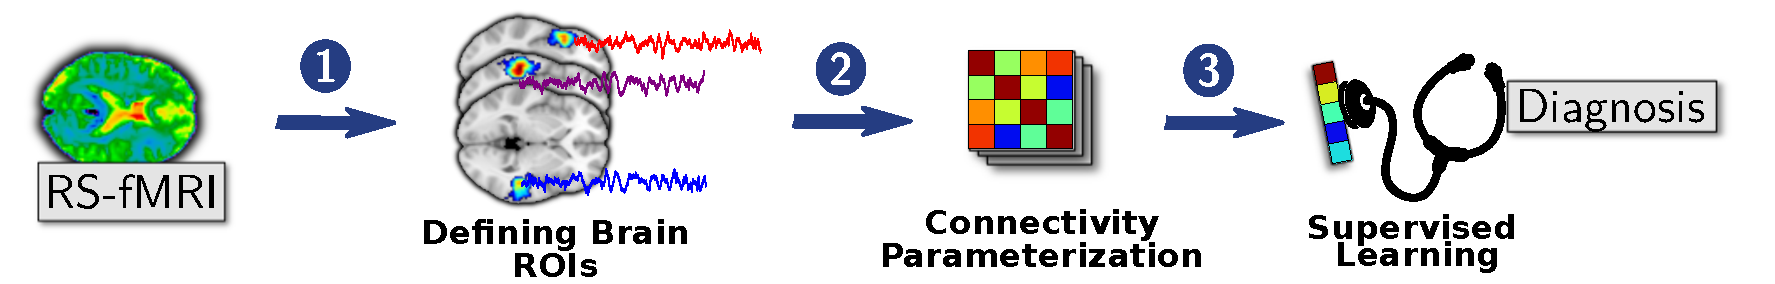
\includegraphics[width=1\linewidth]{figures/functional_connectivity_pipeline.pdf}
\end{center}
\captionof{figure}{\textbf{Our pipeline consists of three main steps}: defines regions
    from rest fMRI,
    builds connectomes from time series signals extracted from these
    regions of interests, and compares connectomes across subjects using
machine learning. \label{fig_1}}
%\vspace{\figurespace}


\vspace{0.6\sectionspace}
\section{Rest fMRI datasets}

\begin{center}
    \begin{tabular}{ccc}
        \rowcolor{gray!50}
        Dataset & Subjects & Clinical question \\
        \hline\\[-4mm]
        COBRE & $65/77$ & Schizophrenia vs Control \\
        \rowcolor{gray!13}
        ADNI & $40/96$ & AD vs MCI  \\
        ADNIDOD & $89/78$& PTSD vs Control \\
        \rowcolor{gray!13}
        ACPI & $62/64$ & Marijuana use vs Control \\
        ABIDE & $402/464$ & Autism vs Control
    \end{tabular}
\end{center}
\captionof{table}{Description of the five rs-fMRI
    datasets used.
    AD - Alzheimer's Disease, MCI - Mild
    Cognitive Impairment,
    PTSD - Post Traumatic Stress Disorder.}
%\vspace{\tablespace}

\section{Pipelining choices}
    %\begin{enumerate}
    %   \item Defining Brain ROIs
    %   \item Connectivity parameterizing
    %   \item Supervised Learning: Classifiers
    %\end{enumerate}
%\vspace{\figurespace}
\begin{center}
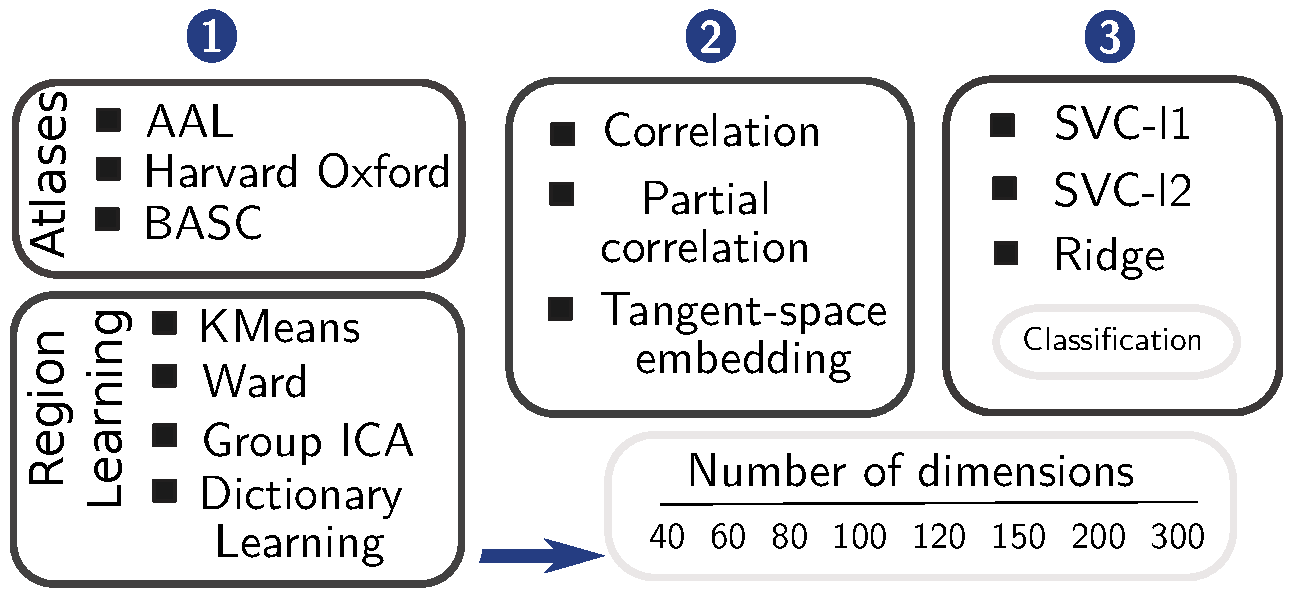
\includegraphics[width=0.7\linewidth]{figures/only_pipeline_choices.pdf}
\end{center}
\captionof{figure}{{\bfseries\sffamily 1 -- Defining Brain ROIs} can be done using
    three pre-defined atlases: two anatomical - Automated Anatomical Labeling
    (AAL), Harvard Oxford and one functional - Bootstrap Analysis
    of Stable Clusters (BASC). Four region learning methods: two Linear
    decomposition models - Group Independent Component Analysis (Group ICA),
    Online Dictionary Learning and two Clustering models - KMeans,
    Agglomerative with Ward criterion.
    {\bfseries\sffamily 2 -- Parameterizing functional connectivity
    between ROIs}: correlation, partial correlation or tangent space embedding
    {\bfseries\sffamily 3 -- Supervised learning}: Classifiers, a
classification
    model is built to predict groups with two linear classifiers, SVC
($\ell_{1}$
    or $\ell_{2}$ penalization) and Ridge. Definition of brain regions (below). \label{fig_2}}
%\vspace{\figurespace}


%\begin{centering}
\begin{minipage}{0.22\textwidth}
\begin{minipage}{1.5\linewidth}
\begin{center}
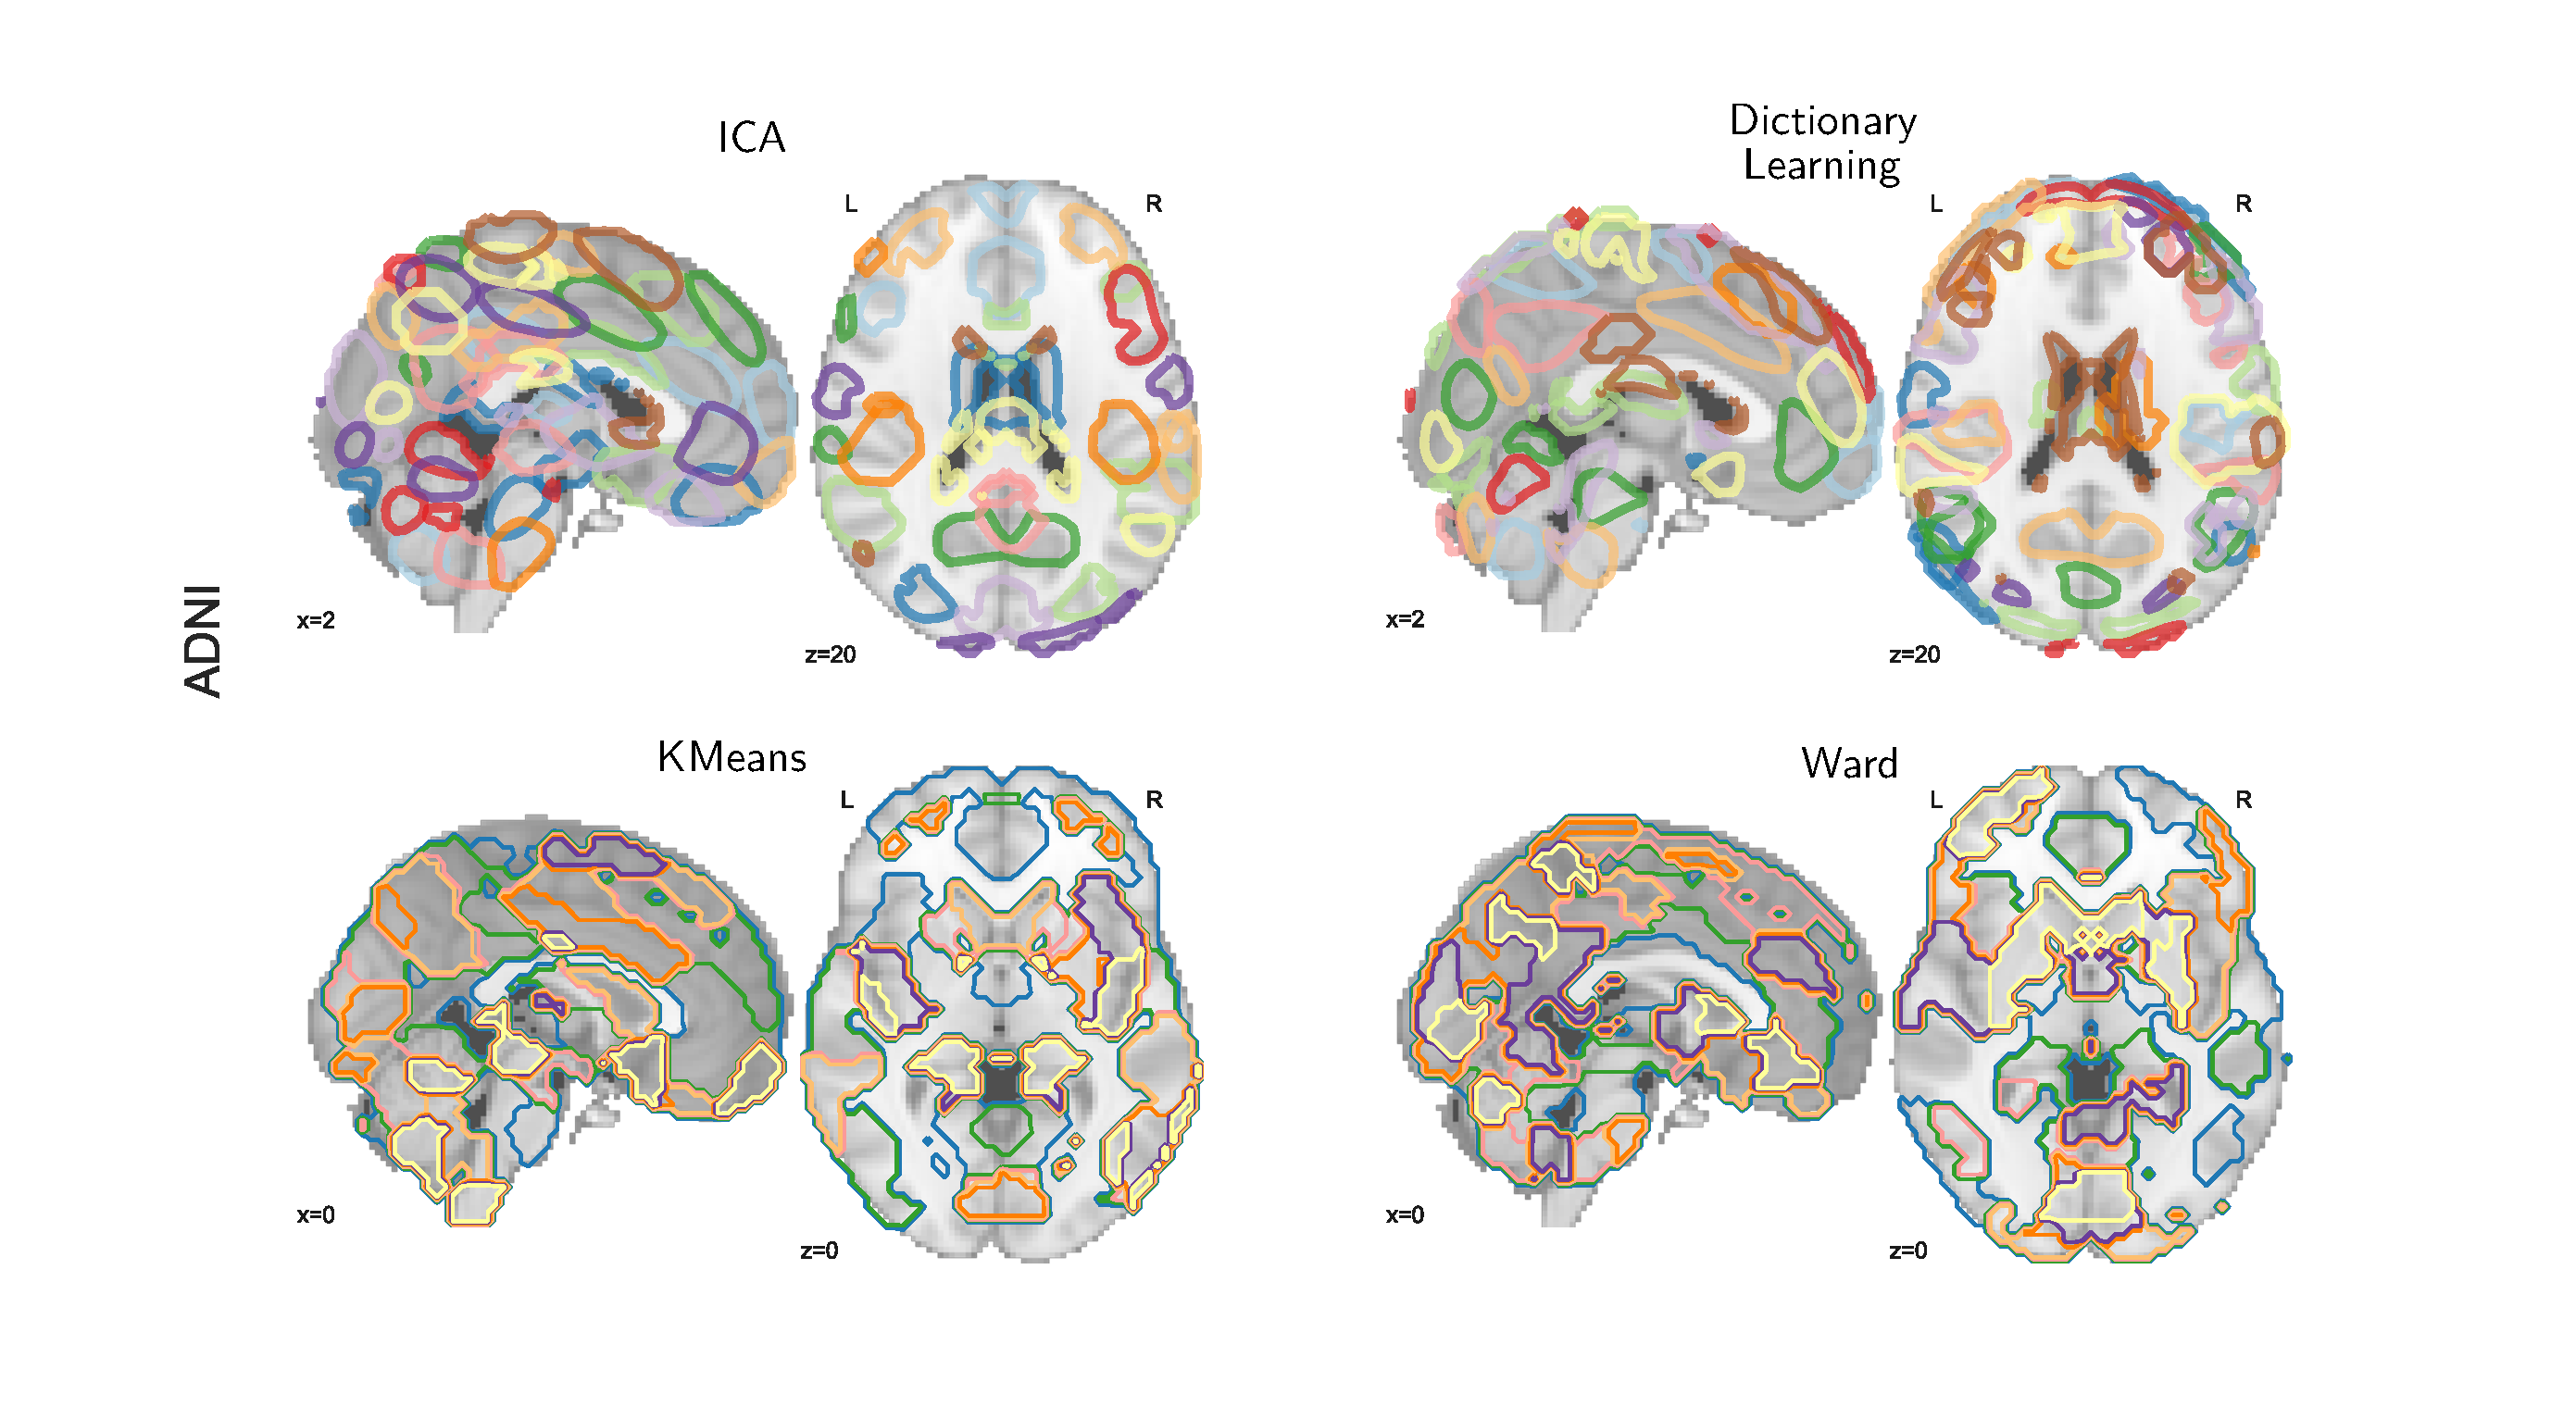
\includegraphics[width=2.22\linewidth]{figures/rois2.pdf}
%\captionof{figure}{Definition of Brain regions. \label{fig_3}}
\end{center}
\end{minipage}
\end{minipage}
%\end{centering}
%\vspace{\figurespace}
%\begin{minipage}[t]{0.35\linewidth}
%        Here is the text
%          \end{minipage}\hfill
%            \begin{minipage}[b]{0.55\linewidth}
%                    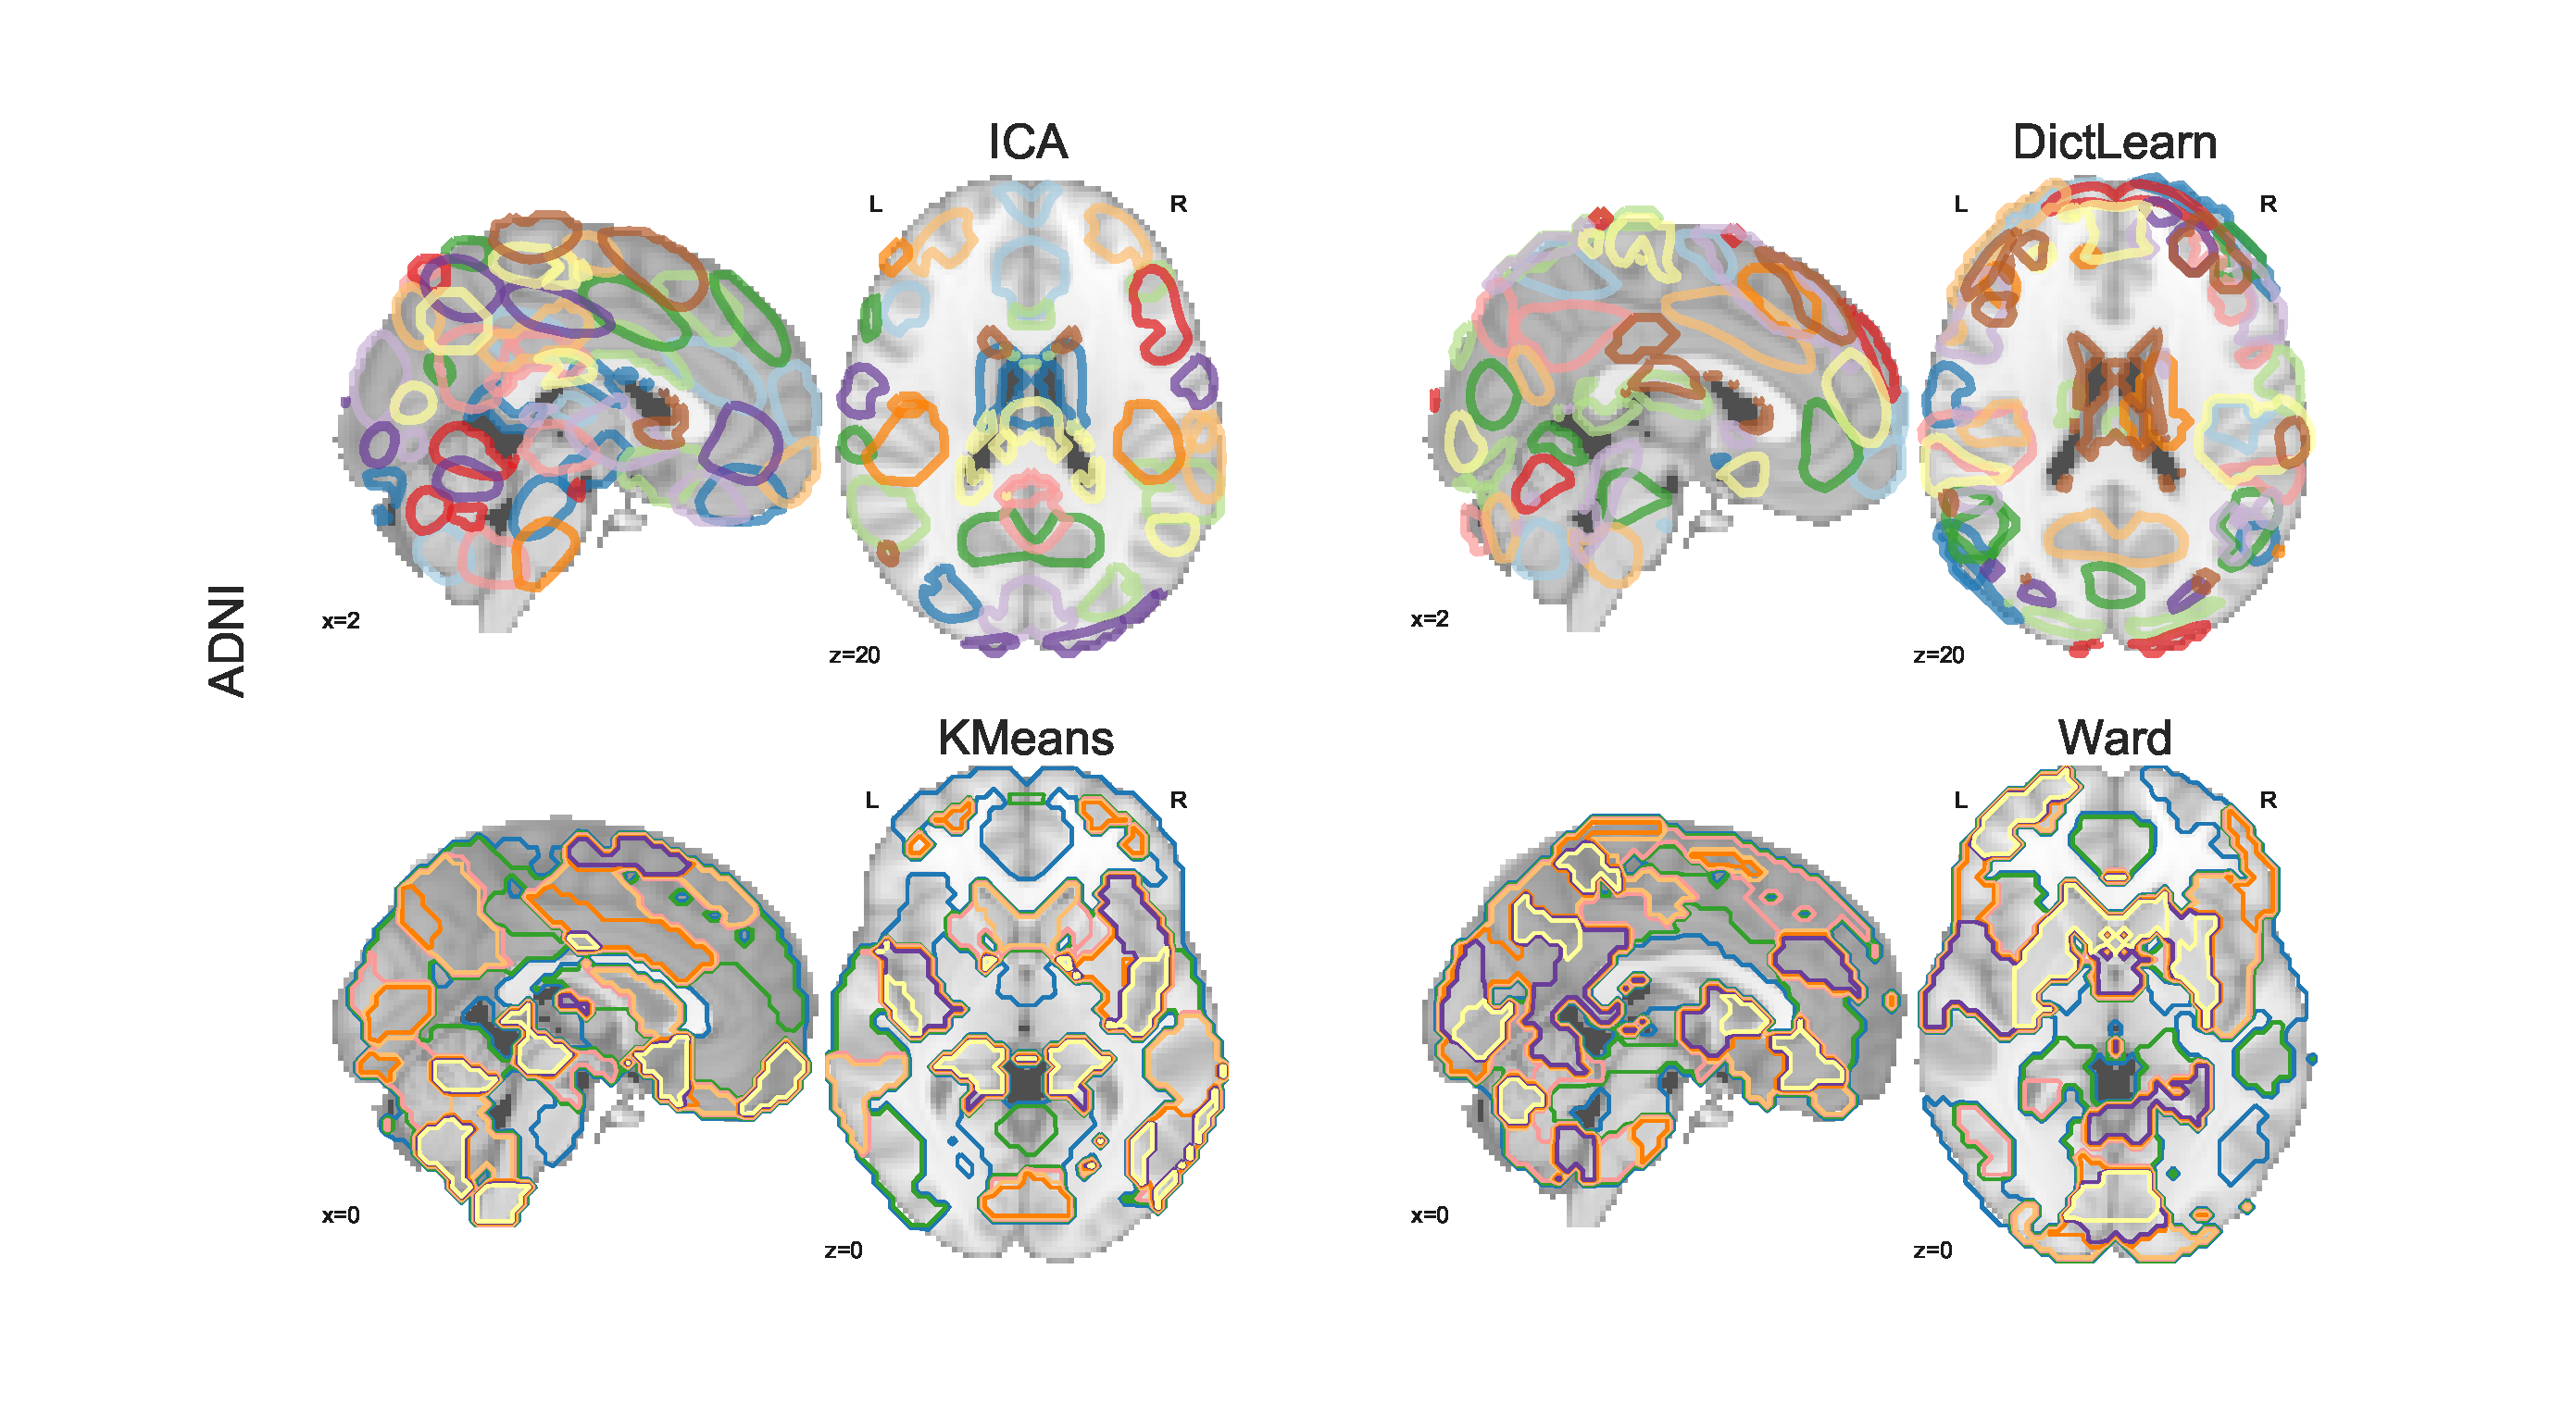
\includegraphics[width=40cm]{figures/rois.pdf}
%                        \captionof{figure}{A wonderful picture}
%                          \end{minipage}
%

% The end of the first column and the start of the second
\end{minipage} % no empty line before the next ''\begin''
\hspace{0.02\linewidth} % Middle margin
\begin{minipage}[t]{0.48\linewidth}
\setlength{\parindent}{10mm} % Paragraph indent










\section{Results}
\subsection{Prediction scores in AUC}
\begin{tabularx}{\textwidth}{p{7.5cm}|p{5.5cm}|p{5.5cm}|p{5.5cm}|p{5.5cm}|p{5.5cm}}
    \rowcolor{gray!50}
    \centering{Accuracy} & \centering{COBRE} & \centering{ADNI} &
    \centering{ADNIDOD} & \centering{ACPI} & ABIDE \\
    \hline
    \rowcolor{gray!13}
    \centering{Median}& \centering{$87.1\%$} & \centering{$76.2\%$} &
    \centering{$67.1\%$} & \centering{$56.4\%$} & $70.2\%$\\
    % \rowcolor{gray!13}%
        {\centering $5^{th}$ Percentile} & \centering{$74.3\%$} &
    \centering{$62.3\%$} & \centering{$53.8\%$} & \centering{$41.4\%$} & $64.9\%$\\
    \rowcolor{gray!13}
    {\centering $95^{th}$ Percentile} & \centering{$94\%$} &
    \centering{$89.1\%$} & \centering{$77.2\%$} & \centering{$68.7\%$} & $73.8\%$\\
    \hline
\end{tabularx}
\captionof{table}{\textbf{Median, 5th percentile and 95th percentile of
        accuracy scores in AUC over cross-validation folds ($n=100$) across
        multi rs-fMRI datasets.} Functional brain atlases learned using Online
        Dictionary Learning\cite{arthur} with $60$ resting state networks
        and spliting networks to regions are used in the prediction pipeline
        with Tangent based connectivity matrix parameterization\cite{varoquaux} and
        Support Vector Classifier with $\ell{_2}$ penalization (SVC-$\ell{_2}$).}

\subsection{Choice of classifier, connectivity and brain atlas}
%\vspace{\figurespace}
\begin{center}
\begin{minipage}[t]{0.48\linewidth}
\begin{center}
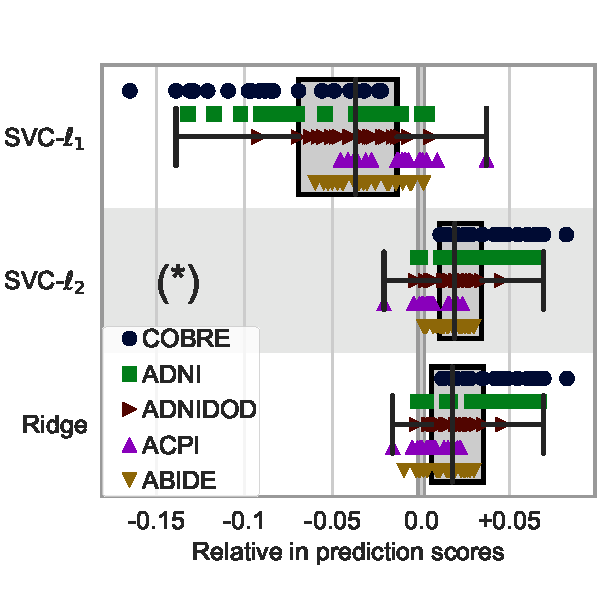
\includegraphics[width=0.95\linewidth]{figures/impact_plot_classifier.pdf}\\\normalsize
(a) classifier
\end{center}
\end{minipage}
\hspace{0.02\linewidth} % Middle margin
\begin{minipage}[t]{0.48\linewidth}
\begin{center}
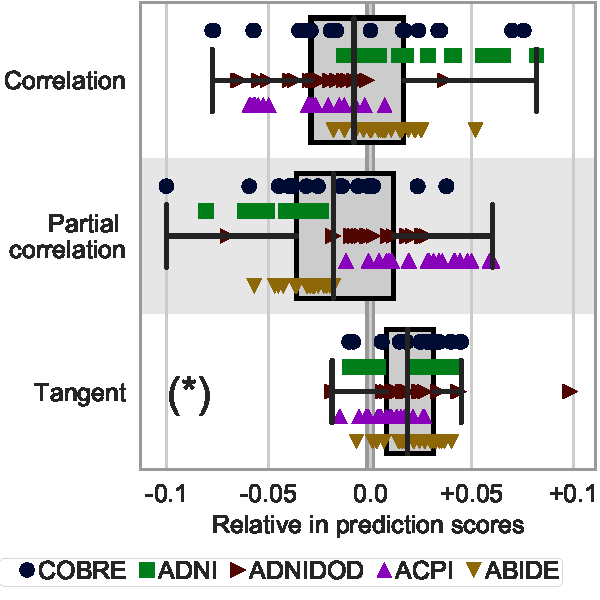
\includegraphics[width=0.87\linewidth]{figures/impact_plot_measure.pdf}\\\normalsize
(b) connectivity parameterization
\end{center}
\end{minipage}
\end{center}
%\captionof{figure}{The impact of classifier (a), connectivity
%parameterization (b)
%            choices in functional connectivity prediction pipeline over
%                    diverse tasks. \label{fig_3}}
%\vspace{\figurespace}

%\subsection{Choice of atlas}
%\vspace{\figurespace}
\begin{minipage}[t]{0.98\textwidth}
\begin{center}
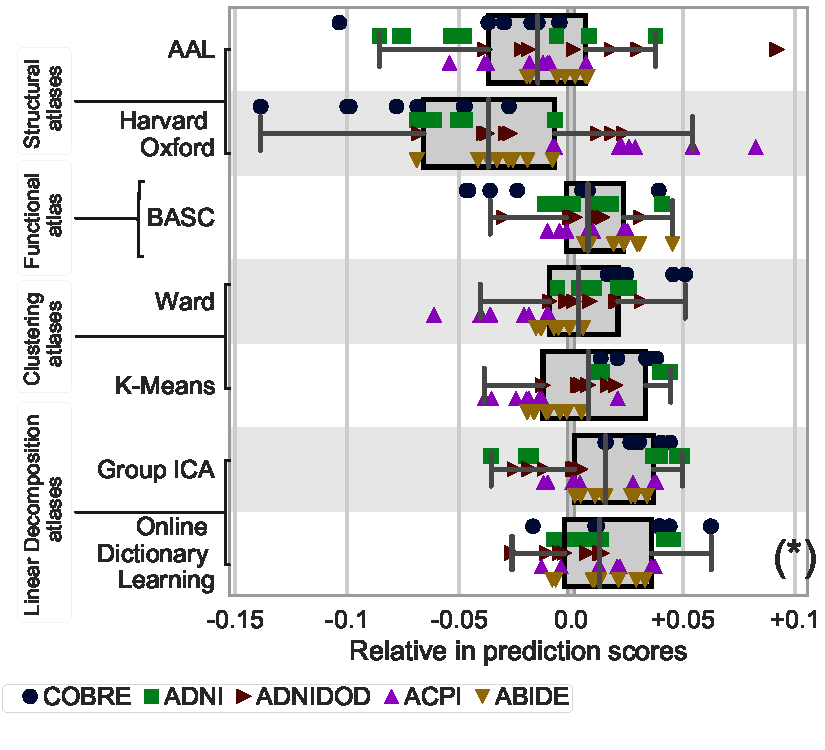
\includegraphics[width=0.8\linewidth]{figures/impact_plot_atlas.pdf}\\
\normalsize (c) brain atlases with optimal choices in dimensionality
-- BASC (122 networks to regions) -- Ward (120) --
K-Means (120 parcellations) --
GroupICA (80 networks to regions) -- DictLearn (60 networks to regions)
%\vspace{\figurespace}
\end{center}
\end{minipage}
\captionof{figure}{The \textbf{impact of choices} in functional connectivity prediction
    pipeline over diverse tasks.
    (*) indicates the optimal option.
        \label{fig_3}}

%\vspace{\sectionspace}
\section{Optimal choices}
\begin{itemize}
    %\item Functional-Connectivity based pipeline across diverse clinical targets
    \item Systematic exploration of choices at each step
    \item Definition of Brain ROIs - Linear Decomposition models
    \item Connectivity Parameterization - Tangent Space Embedding
    \item Classification with Support Vector Classifier - $\ell{_2}$
        penalization.
\end{itemize}

\nocite{*}
%\vspace{\sectionspace}
\begin{spacing}{0.6}
\bibliographystyle{naturemag}
\bibliography{references}
\end{spacing}










\end{minipage}
\end{minipage} % minipage for the two columns (minipages)










\vfill % Fill the free space until the footer minipages










\begin{minipage}{0.98\textwidth} % Minipages for the footers

\large % Text size for footers

\begin{minipage}[c]{0.475\linewidth}% Footer #1
\vspace{0pt}
\begin{center}
\textcolor{posterGray}{\hrule}
\vspace{0pt}

\includegraphics[height=17mm, angle=0]{figures/logos/parietal_web_page.png}
\qquad \quad

\includegraphics[height=17mm, angle=0]{figures/logos/neurospin.jpg}
\qquad \quad

\includegraphics[height=29mm, angle=0]{figures/logos/logo-inria2.jpg}
\end{center}
\end{minipage} % No empty line before the second begin!
\hspace{0.01\linewidth}
\begin{minipage}[c]{0.575\linewidth} % Footer #2
    \begin{center}
\vspace{0pt}
\textbf{\sffamily Acknowledgments:}\\
ANR-11-BINF-0004\_NiConnect and
CATI project.
\end{center}
\end{minipage}

\end{minipage}





\vspace*{0.03\linewidth} % Increase the bottom margins





\end{document}
